%%% The main file. It contains definitions of basic parameters and includes all other parts.

%% Settings for single-side (simplex) printing
% Margins: left 40mm, right 25mm, top and bottom 25mm
% (but beware, LaTeX adds 1in implicitly)
\documentclass[12pt,a4paper]{report}
\setlength\textwidth{145mm}
\setlength\textheight{247mm}
\setlength\oddsidemargin{15mm}
\setlength\evensidemargin{15mm}
\setlength\topmargin{0mm}
\setlength\headsep{0mm}
\setlength\headheight{0mm}
% \openright makes the following text appear on a right-hand page
\let\openright=\clearpage

%% Settings for two-sided (duplex) printing
% \documentclass[12pt,a4paper,twoside,openright]{report}
% \setlength\textwidth{145mm}
% \setlength\textheight{247mm}
% \setlength\oddsidemargin{14.2mm}
% \setlength\evensidemargin{0mm}
% \setlength\topmargin{0mm}
% \setlength\headsep{0mm}
% \setlength\headheight{0mm}\textsl{•}
% \let\openright=\cleardoublepage

\usepackage{colorprofiles}

%% Generate PDF/A-2u
\usepackage[a-2u]{pdfx}

%% Character encoding: usually latin2, cp1250 or utf8:
\usepackage[utf8]{inputenc}

%% Prefer Latin Modern fonts
\usepackage{lmodern}

%% Further useful packages (included in most LaTeX distributions)
\usepackage{amsmath}        % extensions for typesetting of math
\usepackage{amsfonts}       % math fonts
\usepackage{amsthm}         % theorems, definitions, etc.
\usepackage{bbding}         % various symbols (squares, asterisks, scissors, ...)
\usepackage{bm}             % boldface symbols (\bm)
\usepackage{graphicx}       % embedding of pictures
\usepackage{fancyvrb}       % improved verbatim environment
\usepackage{natbib}         % citation style AUTHOR (YEAR), or AUTHOR [NUMBER]
\usepackage[nottoc]{tocbibind} % makes sure that bibliography and the lists
			    % of figures/tables are included in the table
			    % of contents
\usepackage{dcolumn}        % improved alignment of table columns
\usepackage{booktabs}       % improved horizontal lines in tables
\usepackage{paralist}       % improved enumerate and itemize

% Packages added by the author of the thesis
\usepackage[threshold=1]{csquotes}


% python-like algorithm environment
\usepackage[ruled,noline]{algorithm2e}

\newcommand{\forcond}{$i=0$ \KwTo $n$}
\SetKwFunction{FRecurs}{FnRecursive}%

\SetStartEndCondition{ }{}{}%
\SetKwProg{Fn}{def}{\string:}{}
\SetKwFunction{Range}{range}%%
\SetKw{KwTo}{in}\SetKwFor{For}{for}{\string:}{}%
\SetKwIF{If}{ElseIf}{Else}{if}{:}{elif}{else:}{}%
\SetKwFor{While}{while}{:}{}%
\renewcommand{\forcond}{$i$ \KwTo\Range{$n$}}
\AlgoDontDisplayBlockMarkers\SetAlgoNoEnd\SetAlgoNoLine%


% TODO notice this line, discuss it
\PassOptionsToPackage{usenames}{xcolor}
% TODO
%\usepackage[usenames]{xcolor}  % typesetting in color

%%% Basic information on the thesis

% Thesis title in English (exactly as in the formal assignment)
\def\ThesisTitle{Evolutionary optimization of machine learning workflows}

% Author of the thesis
\def\ThesisAuthor{Gabriela Suchopárová}

% Year when the thesis is submitted
\def\YearSubmitted{2019}

% Name of the department or institute, where the work was officially assigned
% (according to the Organizational Structure of MFF UK in English,
% or a full name of a department outside MFF)
\def\Department{Department of Theoretical Computer Science and Mathematical Logic}

% Is it a department (katedra), or an institute (ústav)?
\def\DeptType{Department}

% Thesis supervisor: name, surname and titles
\def\Supervisor{Mgr. Roman Neruda, CSc.}

% Supervisor's department (again according to Organizational structure of MFF)
\def\SupervisorsDepartment{Department of Theoretical Computer Science and Mathematical Logic}

% Study programme and specialization
\def\StudyProgramme{Computer Science}
\def\StudyBranch{General Computer Science}

% An optional dedication: you can thank whomever you wish (your supervisor,
% consultant, a person who lent the software, etc.)
\def\Dedication{%
Dedication.
}

% Abstract (recommended length around 80-200 words; this is not a copy of your thesis assignment!)
\def\Abstract{%
Abstract.
}

% 3 to 5 keywords (recommended), each enclosed in curly braces
\def\Keywords{%
{Machine learning} {Evolutionary computing} {Meta-learning} {Workflows}
}

%% The hyperref package for clickable links in PDF and also for storing
%% metadata to PDF (including the table of contents).
%% Most settings are pre-set by the pdfx package.
\hypersetup{unicode}
\hypersetup{breaklinks=true}

% Definitions of macros (see description inside)
%%% This file contains definitions of various useful macros and environments %%%
%%% Please add more macros here instead of cluttering other files with them. %%%

%%% Minor tweaks of style

% These macros employ a little dirty trick to convince LaTeX to typeset
% chapter headings sanely, without lots of empty space above them.
% Feel free to ignore.
\makeatletter
\def\@makechapterhead#1{
  {\parindent \z@ \raggedright \normalfont
   \Huge\bfseries \thechapter. #1
   \par\nobreak
   \vskip 20\p@
}}
\def\@makeschapterhead#1{
  {\parindent \z@ \raggedright \normalfont
   \Huge\bfseries #1
   \par\nobreak
   \vskip 20\p@
}}
\makeatother

% This macro defines a chapter, which is not numbered, but is included
% in the table of contents.
\def\chapwithtoc#1{
\chapter*{#1}
\addcontentsline{toc}{chapter}{#1}
}

% Draw black "slugs" whenever a line overflows, so that we can spot it easily.
\overfullrule=1mm

%%% Macros for definitions, theorems, claims, examples, ... (requires amsthm package)

\theoremstyle{plain}
\newtheorem{thm}{Theorem}
\newtheorem{lemma}[thm]{Lemma}
\newtheorem{claim}[thm]{Claim}

\theoremstyle{plain}
\newtheorem{defn}{Definition}

\theoremstyle{remark}
\newtheorem*{cor}{Corollary}
\newtheorem*{rem}{Remark}
\newtheorem*{example}{Example}

%%% An environment for proofs

%%% FIXME %%% \newenvironment{proof}{
%%% FIXME %%%   \par\medskip\noindent
%%% FIXME %%%   \textit{Proof}.
%%% FIXME %%% }{
%%% FIXME %%% \newline
%%% FIXME %%% \rightline{$\square$}  % or \SquareCastShadowBottomRight from bbding package
%%% FIXME %%% }

%%% An environment for typesetting of program code and input/output
%%% of programs. (Requires the fancyvrb package -- fancy verbatim.)

\DefineVerbatimEnvironment{code}{Verbatim}{fontsize=\small, frame=single}

%%% The field of all real and natural numbers
\newcommand{\R}{\mathbb{R}}
\newcommand{\N}{\mathbb{N}}

%%% Useful operators for statistics and probability
\DeclareMathOperator{\pr}{\textsf{P}}
\DeclareMathOperator{\E}{\textsf{E}\,}
\DeclareMathOperator{\var}{\textrm{var}}
\DeclareMathOperator{\sd}{\textrm{sd}}

%%% Transposition of a vector/matrix
\newcommand{\T}[1]{#1^\top}

%%% Various math goodies
\newcommand{\goto}{\rightarrow}
\newcommand{\gotop}{\stackrel{P}{\longrightarrow}}
\newcommand{\maon}[1]{o(n^{#1})}
\newcommand{\abs}[1]{\left|{#1}\right|}
\newcommand{\dint}{\int_0^\tau\!\!\int_0^\tau}
\newcommand{\isqr}[1]{\frac{1}{\sqrt{#1}}}

%%% Various table goodies
\newcommand{\pulrad}[1]{\raisebox{1.5ex}[0pt]{#1}}
\newcommand{\mc}[1]{\multicolumn{1}{c}{#1}}


% Title page and various mandatory informational pages
\begin{document}
%%% Title page of the thesis and other mandatory pages

%%% Title page of the thesis

\pagestyle{empty}
\hypersetup{pageanchor=false}
\begin{center}

\centerline{\mbox{
\includegraphics[width=166mm]{../img/logo-en.pdf}}}

\vspace{-8mm}
\vfill

{\bf\Large BACHELOR THESIS}

\vfill

{\LARGE\ThesisAuthor}

\vspace{15mm}

{\LARGE\bfseries\ThesisTitle}

\vfill

\Department

\vfill

\begin{tabular}{rl}

Supervisor of the bachelor thesis: & \Supervisor \\
\noalign{\vspace{2mm}}
Study programme: & \StudyProgramme \\
\noalign{\vspace{2mm}}
Study branch: & \StudyBranch \\
\end{tabular}

\vfill

% Zde doplňte rok
Prague \YearSubmitted

\end{center}

\newpage

%%% Here should be a bound sheet included -- a signed copy of the "bachelor
%%% thesis assignment". This assignment is NOT a part of the electronic
%%% version of the thesis. DO NOT SCAN.

%%% A page with a solemn declaration to the bachelor thesis

\openright
\hypersetup{pageanchor=true}
\pagestyle{plain}
\pagenumbering{roman}
\vglue 0pt plus 1fill

\noindent
I declare that I carried out this bachelor thesis independently, and only with the cited
sources, literature and other professional sources.

\medskip\noindent
I understand that my work relates to the rights and obligations under the Act No.~121/2000 Sb.,
the Copyright Act, as amended, in particular the fact that the Charles
University has the right to conclude a license agreement on the use of this
work as a school work pursuant to Section 60 subsection 1 of the Copyright Act.

\vspace{10mm}

\hbox{\hbox to 0.5\hsize{%
In ........ date ............	% FIXME!
\hss}\hbox to 0.5\hsize{%
signature of the author
\hss}}

\vspace{20mm}
\newpage

%%% Dedication

\openright

\noindent
\Dedication

\newpage

%%% Mandatory information page of the thesis

\openright

\vbox to 0.5\vsize{
\setlength\parindent{0mm}
\setlength\parskip{5mm}

Title:
\ThesisTitle

Author:
\ThesisAuthor

\DeptType:
\Department

Supervisor:
\Supervisor, \SupervisorsDepartment

Abstract:
\Abstract

Keywords:
\Keywords

\vss}

\newpage

\openright
\pagestyle{plain}
\pagenumbering{arabic}
\setcounter{page}{1}


%%% A page with automatically generated table of contents of the bachelor thesis

\tableofcontents

%%% Each chapter is kept in a separate file
\chapter*{Introduction}
\addcontentsline{toc}{chapter}{Introduction}

Over the last few years we have witnessed an enormous success of the artificial
intelligence. Thanks to advances in machine learning, a great variety of
applications emerged, ranging from automatized analyses of documents, through
image recognition to music recommendation. The artificial intelligence is already
influencing many parts of our everyday lives.

However, most of these examples rely on fine tuned models developed by large
teams of experts. In addition, a lot of time and resources is necessary. These
factors make the machine learning off-limits to non-experts from unrelated
fields. % maybe sth about finances
\chapter{Preliminaries}

%An~example citation: \cite{Andel07}
\textit{What we will talk about, theory}

\section{Machine learning}
The field of machine learning encompasses a broad range of algorithms and
statistical methods for data processing. In his book on machine learning,
Flach provides the following general definition:

\blockquote{Machine learning is the systematic study of algorithms and systems
that improve their knowledge or performance with experience.
(\cite{Flach:2012:MLA:2490546})} % page number? (3)
%
% Here a detailed definition
%
The knowledge of a system is gained through learning from \emph{experience}.
This procedure is referred to as the \emph{training} phase. In this process, 
the algorithm adjusts its parameters according to the nature of training data.
The result of the process is a prediction function which depends on learned
parameters. By applying this function on previously unseen data, denominated 
as the \emph{testing} data, we obtain the output of the algorithm. The 
result is then evaluated to determine the performance of the method. 
(\cite{Bishop:2006:PRM:1162264}) The character of the learning process
varies with different machine learning problems. There are three main classes 
of tasks: \emph{supervised}, \emph{unsupervised} and \emph{reinforcement} 
learning.
% This should be improved

In case of supervised learning, the training data is a set of labelled examples
and the task is to predict labels of previously unseen data. The field is 
further subdivided into two groups. If the labels are elements of a finite 
number of discrete categories, the problem is called \emph{classification}. 
The continuous case is then called \emph{regression}.
% This is Bishop as well... TODO cite pages
In contrast to supervised learning, in unsupervised learning the training data 
is unlabelled. The key task is therefore to divide the data into groups of 
similar examples. The task of reinforcement learning is to find suitable actions as to maximize 
a reward. The training data is typically some history of previous actions 
and corresponding rewards.

It is important to note that good performance on training data does not ensure 
just as good performance on new data. Sometimes the model performs 
exceptionally well on training data, but fares much worse on testing data. 
This behaviour is called \emph{overfitting} and usually occurs when 
unnecessarily subtle details of the data are learned. The opposite concept 
is called \emph{generalisation}, which is the ability to perform well on 
different types of testing data.

A related term is the so-called `\emph{bias-variance dilemma}'. A 
low-complexity model will not overfit, but a lot of errors will be made, thus 
introducing a certain bias from the correct output. On the other hand, by 
increasing the number of model parameters, it will highly depend on training 
data. Then, with small changes in data there will be a high variance in 
output. A balance can rarely be achieved in practice, hence it is often 
necessary to choose the side that is less harmful to the task. Another option
is to use some of the ensemble methods described in \ref{ensemble}. For
example, \hyperref[bagging]{bagging} is a method of variance reduction, while
\hyperref[boosting]{boosting} noticeably reduces the bias. More on this topic
can be found in Flach's book. (\citet[p.~93--94,~338]{Flach:2012:MLA:2490546})

% here more on supervised learning, hypotheses,...

\subsection{Model ensembles} \label{ensemble}
% Mention netflix like they did in the paper?
% Find sources where they mention successful applications
Model ensembles are powerful learning techniques that combine simpler models 
to achieve better results. They are widely used in practice, specific examples
can be found in the review of \cite{Rokach:2009:TCE:1609202.1609436}.

The rationale behind ensembles is also of theoretical character, namely from
statistics and from computational learning theory. In statistics, a general
idea is to average measurements to get more stable and reliable results.
Here, the models are trained on data samples or feature subsets and the results
are then combined into a final hypothesis.
% Flach

% Variant A, possibly inacurrate
The computational learning theory defines the term \emph{learnability},
which describes whether a model outputs a correct hypothesis by learning on
random sets of instances from a unknown distribution. A \emph{strong learner}
is a model which outputs most of the time a correct hypothesis. It is not
required that it always produces a hypothesis with error equal to zero, as 
the set of chosen instances might be atypical or not representative enough.
Similarly, a \emph{weak learner} is then a model which outputs most of the time
a hypothesis, which is slightly better than random guessing (i.e. has a
success rate over 0.5). A more detailed elaboration of the learnability
theory is beyond the scope of this work and can be found in books 
of \citep{Flach:2012:MLA:2490546} and \citep{Mitchell:1997:ML:541177}.

% Variant B, possibly tedious to read
%The computational learning theory defines the term \emph{learnability},
%which describes whether a concept language can be reliably learnt. A concept is
%defined as a logical expression which describes a set of instances. A 
%hypothesis space is then the space of possible concepts.

%Having a model $M$ and a concept language $C$, $C$ is (strongly)
%\emph{PAC-learnable} by $M$ if the model outputs most of the time a hypothesis 
%with a very small error. The model is not required to be correct every time, 
%as the set of chosen instances described by the language might be atypical 
%or not representative enough.  We can also define the \emph{weak learnability} 
%of $C$ by $M$ where $M$ outputs a hypothesis which is slightly better than 
%random guessing (i.e. success rate over 0.5). 

The assumption of strong learnability may appear to be quite strict when 
compared to the weak learnability, as the model must output a correct 
hypothesis on almost all example sets. However, Shapire proved that a model 
is weakly learnable if and only if it is strongly learnable. 
\citep{Schapire:1990:SWL:83637.83645} This was proven in a constructive manner
by iteratively correcting the errors of the hypotheses, thus \emph{boosting} 
the model. The boosting method has directly inspired one of the most successful
ensemble methods --- the award winning AdaBoost.
\cite{Freund:1996:ENB:3091696.3091715, Freund:1997:DGO:261540.261549}

In the following sections, we will present some of the most used ensemble 
methods.
\phantomsection
\paragraph{Bagging} \label{bagging}
\emph{Bootstrap aggregating}, usually abbreviated to bagging, is a highly
effective ensemble method. First, $n$ samples are independently taken from 
the original dataset with replacement. This is referred to as 
\emph{bootstrapping}. Then, we use the samples to train an ensemble of $n$
different models. It can be then used to generate predictions, which can be
then \emph{aggregated} by voting or averaging.

This method takes advantage of the statistical stability described at the
beginning of this section. As the examples are drawn with replacement, there
will be some instances missing in every sample. Thus, we introduce diversity
between the ensemble models. \citep[331]{Flach:2012:MLA:2490546}

\phantomsection
\paragraph{Boosting} \label{boosting}
The above-mentioned boosting technique uses a different approach to model
combining. Before the learning process starts, we add weights to the training 
examples (the base-learner must support weighting). Then, we learn the model
on the modified training set, which produces a set of misclassified instances
along with the (weighted) training error. We then adjust the weights in such a
way that weights of the correctly classified examples decrease and those of
the incorrectly classified examples increase. Therefore, when we continue and
learn a new model on the data with changed weights, it will concentrate more 
on the problematic instances.

The algorithm stops after a fixed number of iterations or when the weighted
training error increases over $0.5$ --- which is when the algorithm stops
improving. The resulting prediction is again an average of all model
predictions, but with putting more weight on models with a lower training
error. \citep[335]{Flach:2012:MLA:2490546}

\section{AutoML}
When using machine learning in practice, it is not always evident which model
is suitable for a particular problem. Moreover, there is a vast number of model
and parameter combinations to choose from, not to mention model ensembles.
Furthermore, it is necessary to preprocess the data and construct features
for the learning process. All these aforementioned tasks require human 
expertise and are typically time-consuming. AutoML aims to automatize the
process and make machine learning available to non-experts.
% todo internet source - AutoML page

% Goals - what, how, why
There seems to be no generally accepted definition of AutoML as for now.
According to \cite{DBLP:journals/corr/abs-1810-13306},
\textquote{\textit{AutoML attempts to construct machine learning programs
\ldots without human assistance and within limited computational budgets.}}
Informally, AutoML encompasses methods that automatize a part of a machine
learning workflow. Examples of existing methods are presented in chapter
\ref{ch2:related}.

\subsection{Machine learning workflows}
A machine learning workflow is the process of solving a particular machine
learning problem. In literature, it is also labelled as a `machine learning
pipeline' \cite{DBLP:journals/corr/abs-1810-13306}. However, in the context
of AutoML it may not be a suitable term, as a pipeline is a linear acyclic
graph and some parts of the flow may by cyclic, as can be seen
in figure \ref{pic01:workflow}.

\begin{figure}[h]\centering
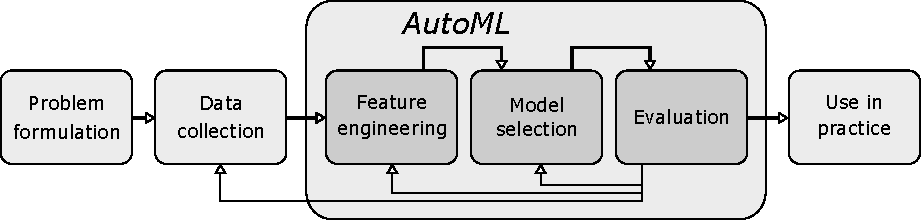
\includegraphics[width=\textwidth]{../img/workflow-pdfa.pdf}
\caption{A typical machine learning workflow}
\label{pic01:workflow}
\end{figure}

The process of solving the problem is iterative; it is usually necessary to try
out many different settings, as there are no algorithms that would perform
well on all types of problems.
There are many possibilities in what to optimize. Some models concentrate only
on one part of the workflow, for example on automatic feature engineering,
other handle multiple steps at once. As mentioned above, there is no general
categorization % hierarchy? better word
of AutoML frameworks. Thus, in the following sections we present only some
AutoML approaches relevant to this work. For more examples and a proposition
of a general AutoML framework refer to \cite{DBLP:journals/corr/abs-1810-13306}.

% Model creation
%    Architecture  \_ CASH - combined algorithm selection and hyperparams
%    Parameters    /  + AutoML for arbitrary size pipes
%                         - except for TPOT trees and ML-plan
%                           (hieararchical task networks)

% Model recommendation
%    Metalearning

% Combining both - my GP,... (maybe auto-sklearn)

% or CASH
\subsection{Hyperparameter optimization}
Automated hyperparameter optimization (HPO) is the most basic, but nevertheless
very important task of AutoML. As has already been mentioned, there is no
silver-bullet method that would solve all machine learning problems.
Furthermore, every method depends on some hyperparameters that greatly
influence its performance. Combining this, we get a large search space of
possible models. This problem is called]
\emph{combined algorithm selection and hyperparameter optimization problem}
(CASH) and a formal definition can be found in
\citep{DBLP:journals/corr/abs-1208-3719}.

There are several limitations which complicate the search through this space.
For large models (for example in deep learning) and large dataset, the
learning process and evaluation take a lot of time. Moreover, the
configuration space may be quite complex, with many continuous hyperparameters
which also depend on each other. It is also necessary to avoid overfitting,
which is not always obvious as the training set may not be large enough.

Some examples of frameworks which try to solve the HPO are mentioned in section
\ref{ch2:related}. Various approaches are presented in the book written by
\cite{automl_book}.

\subsection{Creating model architecture}
\textit{NAS, arbitrary sized pipes}

\subsection{Metalearning}
The metalearning, also known as `learning to learn' \ldots

Just as the traditional learning --- here referred to as \emph{base-learning}
--- metalearning improves with experience. The difference lies in the learning
process. While base-learning comprises of a single run on a specific task,
metalearning may include several runs or many different tasks.

In the research area of model recommendation, the training data is most
frequently a history of previous runs. A suitable model is then chosen by
examining which models were successful on similar tasks. As the problem data
may differ significantly, the tasks cannot be usually compared directly.
Therefore, we need to accumulate some kind of \emph{metaknowledge} which
can be extracted even from substantially different data.

\textit{Describe meta-data, meta-features, compare to EVA approach.}
% also describe specific meta ensembles

\section{Evolutionary computing} \label{ea}
Evolutionary computing is a heuristic optimization method inspired by 
Charles Darwin's theory of \emph{natural selection}. \cite{darwin} In 
a population, individuals with the best characteristics are most likely
to reproduce, thus passing the traits to the offspring. As the 
evolution is repeated over several generations, the most advantageous traits 
predominate. This phenomenon is also called `survival of the fittest'.

In an evolutionary algorithm, the goal is to find the ``best'' solution 
to the given problem by optimizing a \emph{objective function}. The term
`population' refers to a set of solutions encoded as chromosomes which 
represent the defining features of a particular solution. This corresponds
to the genotype--phenotype relationship from genetics. The `natural selection'
can be then understood as a stochastic search through the space of possible 
chromosome values. 
(\cite{Engelbrecht:2007:CII:1557464})

\textit{exploration vs exploitation...}

% Maybe a better section name
\subsection{Evolutionary algorithms in detail}
As can be seen in algorithm \ref{alg:EA}, a genetic algorithm should 
define a suitable \emph{selection} method, \emph{mutation} and/or 
\emph{crossover} operators and a \emph{fitness function}.
The algorithm terminates when some \emph{stopping condition} is met. 

\paragraph{Selection}
The selection may be divided into two steps. The first is the 
\emph{parent selection}, also called \emph{mating selection}
(line \ref{parent:sel}), and the second is called
\emph{environmental selection} or \emph{recombination} (line \ref{envir:sel}).
Sometimes the latter is omitted, as the selection can be limited to copying 
all offspring to the new population.

The purpose of the parent selection is to select individuals for the
mating process. Usually, it is a probabilistic process with `better'
individuals being more likely to be selected. The worse individuals have some
chance to be selected as well for the sake of maintaining diversity in the
population. An example of the mating selection is the
\emph{tournament selection}, where individuals `compete' in rounds and the
overall winner is selected. A round is won by an individual, if it has a 
greater fitness value.

The environmental selection is used to create a new 
population. Unlike the mating selection which is a stochastic process,
replacement is usually deterministic. Individuals with a higher fitness are
usually preferred as in the first type of selection, but the decision may take 
into account the age of the individuals. As such, it is possible to include 
or not to include the parents along with the offspring. A popular option is to 
directly choose a small number of the most successful individuals. This method 
is called \emph{elitism} \citep{Eiben:2015:IEC:2810085}.
An example of an elitist selection algorithm is NSGA-II, which
is described in section \ref{nsgaii}.
% TODO cite pages directly, when citing from a single source for several
% paragraphs

\paragraph{Crossover and mutation}
The crossover and mutation (also called reproduction operators
\citep{Engelbrecht:2007:CII:1557464}) are genetic operators that modify the
structure of individuals to create new ones. Both operations are highly
dependent on problem encoding, as they directly alter the genomes. An example
of the operators can be found in section \ref{gp:treebased}. In the schema 
of the \hyperref[alg:EA]{evolutionary algorithm}, reproduction operators
are applied on parents selected by the mating selection, as can be seen on 
lines \ref{crossover} and \ref{mutation}.

During the crossover, the genetic information of the parents is combined into
one or more children. Most usually, two parents are used to produce two
offspring, though the counts may differ in some special types of evolutionary
algorithms. Ideally, if we have two parents with different but nevertheless
`good' features, the offspring receives both of them.
\citep{Eiben:2015:IEC:2810085}

The mutation is a stochastic operator which is used to introduce diversity into
the population. The structure of the genome is randomly changed in the hope
of creating a more fit individual. Thus, it must be applied with care, as it is
also possible that some good part may be distorted in the process. This can be
avoided by setting a low mutation probability or by elitism.

\paragraph{Stopping criteria}
Some commonly used stopping criteria, as listed by Engelbrecht, are for example 
a limit on the number of generations, a objective function threshold or
termination after no improvement is observed.
(\citep{Engelbrecht:2007:CII:1557464})

% Ze mame ruzny metody, co to delaj ruzne, konkretni popiseme v nasem reseni
% jednobodovy apod nepsat, spis to trochu uzavrit

% ocislovat radky, odkazovat na ne, zakladni prvky jsou
\begin{algorithm} \label{alg:EA}
\DontPrintSemicolon
\caption{Evolutionary algorithm}
  \KwData{population size $k$, stopping condition $c$, 
          crossover probability $p_{cx}$ and mutation probability $p_{mut}$}
  \KwResult{evolved individuals}
  \;
  $P(0) \longleftarrow$ population of size $k$

  \While{$c$ is not met}{
      \For{individual $ind$} {
         compute fitness $f(ind)$
      }
      \For{i in \Range{$k/2$}} {
         $i_1, i_2 \longleftarrow$ select two individuals from $P(n)$\label{parent:sel}

         \If{$p_{cx}$} {
            $crossover(i_1, i_2)$ \label{crossover}
         }
         
         \If{$p_{mut}$ for $k=1,2$} {
            $mutation(i_k)$ \label{mutation}
         }
         \;
         add $i_1, i_2$ to offspring population $P_o(n)$
      }
      \;
      $P(n+1) \longleftarrow$ select $k$ individuals from $P_o(n)$ \label{envir:sel}
  }
  \;
  return $P(c)$  
\end{algorithm}

The advantage of genetic algorithms is such that there are potentially 
many different solutions present in every population. With well defined 
selection and fitness, the algorithm performs a multi-directional search. 
In comparison with other directed search methods, this proves to be a more 
robust approach. (\cite{Michalewicz:1996:GAD:229930}, 
\cite{Mitchell:1997:ML:541177}) % Mitchell page 260

\subsection{Multi-objective optimization} \label{moo}
In many problems, the quality of the solution depends on more than one
objective function. With this, it is much harder to say whether one solution
is strictly better than another. Multi-objective optimization (MOO) formally
describes this class of problems. We first define the general terminology
and then present MOO in evolutionary computation.

In an optimization problem, the task is to maximize or minimize the objective
function $f(x)$, where $x$ is a vector from the search space. The problem may
also be restricted by constraints in the form of equalities and inequalities.
In multi-objective optimization, the setting remains the same, but the
objective function changes to an \emph{objective vector} ---
for objective functions $f_i(x), i = 1,\ldots,k$, the objective vector is 
defined as $f(x)~=~(f_1(x), f_2(x), \ldots, f_k(x))$.

Although the problem setting is similar, the meaning of optimality needs to 
be redefined. For once, given a pair of solutions, one solution may be better 
than the other solution in one objective function and worse in another. For 
this purpose, we need the following definition.

\begin{definition}[Domination]
In a minimization problem, a vector $x_1$ dominates a vector $x_2$ if and 
only if 
\begin{compactitem}
\item $\forall i=1,\ldots,k: f_i(x_1) \leq f_i(x_2)$, and
\item $\exists j=1,\ldots,k: f_j(x_1) < f_j(x_2)$
\end{compactitem}
\end{definition}

As it is possible to have solutions where neither one dominates the other,
it is impossible to determine one optimal solution. Hence we define the 
\emph{Pareto-optimality}
\citep[p.~551-561,~569--573]{Engelbrecht:2007:CII:1557464}.

\begin{definition}[Pareto-optimality]
A vector $x_1$ is said to be \emph{Pareto-optimal}, if there is no other vector
$x_2$ that dominates it. The \emph{Pareto-optimal set} $P^*$ is the set of all
non-dominated solutions. Finally, the \emph{Pareto-optimal front} (Pareto front)
is defined as
$PF^* =\{\, f=(f_1(x^*),\ldots f_k(x^*)) \mid x^* \in P^* ) \,\}$. 
\end{definition}

If we use evolutionary computation to solve multi-objective problems, the
algorithm needs to be modified. As not every individuals are directly
comparable, we cannot use the selection operators defined in
\ref{ea}. As such, there are various approaches on how to solve this problem,
which can be divided into three groups:

\begin{compactitem}
\item Weighted aggregation --- define a single objective function as a weighted
sum of sub-objectives and proceed with standard evolutionary algorithm
\item Population-based non-Pareto solutions --- works with the sub-objectives,
but does not use the dominance
\item Pareto-based solutions --- tries to approximate the Pareto front
\end{compactitem}

From these three groups, we describe in more detail one Pareto-based algorithm.
More examples are presented in 
\cite[p.~170-173]{Engelbrecht:2007:CII:1557464}.
The algorithm is called Nondominated sorting genetic algorithm (NSGA). It is a
\emph{ranking} selection, which means that individuals are sorted by their
fitness values and the selection is performed with regard to the ordering.

To compute the fitness, the individuals are divided into non-dominated fronts.
This is done by finding a Pareto front of a subpopulation, assigning a
front number to its individuals and removing the from the subpopulation.
The process is repeated with front numbers increasing until no unassigned
individuals remain. Every front then obtains a dummy fitness value, where
the fitness of a front $F(n)$ is better than the fitness of $F(n+1)$. Moreover,
for every individual the value is divided by a \emph{niching} factor (while
keeping the fitness inequality). The 
niching factor is defined as
$$N(i)=\sum_{j\neq i}{S(d((i,j))}$$ where 
\begin{equation}
    S(d(i,j))=
    \begin{cases}
      1 - (\dfrac{d(i,j)}{\sigma_{share}})^2, & \text{if}\ d(i,j) < \sigma_{share} \\
      0, & \text{otherwise.}
    \end{cases}
\end{equation}
This is the definition from the original article of
\cite{Srinivas:1994:MOU:1326668.1326671}, but it can be computed in a different
manner, for example as the count of individuals closer than $\sigma_{share}$
\citep{Engelbrecht:2007:CII:1557464}.

\label{nsgaii}
As the algorithm has some drawbacks, like dependence on $\sigma_{share}$,
a very high computational complexity and lack of elitism, the authors of
NSGA have proposed an improved variant called NSGA-II. This algorithm not only
adresses the above-mentioned problems, it also outperforms other elitist
algorithms \citep{Deb:2002:FEM:2221359.2221582}.


\section{Genetic programming}
% TODO GP and dev-GP applications
In this section, we present a subfield of evolutionary computing --- 
the genetic programming (GP) --- where the population is a set of computer 
programs. The aim of this technique is to evolve programs that provide 
a good solution to the given problem. There are various approaches in means 
of how to represent the individuals and what kind of genetic operators to 
use.

\subsection{Tree-based genetic programming} \label{gp:treebased}
The individuals are most frequently represented in the form of 
\emph{syntax trees}. Inner nodes of the tree are \emph{functions}, whereas 
leaves  are constants (\emph{terminals}) and variables. Together, all possible
functions and terminals form the \emph{primitive set}. Every function of the
set must have a well-defined arity value.

An extension of the genetic programming is \emph{strongly typed GP}. It
constraints the primitive set in such a way that every primitive has an output
type and furthermore every function defines input types of its arguments.

The initialization step is very important, as
there are many different ways how to design trees. Also, specialized genetic
operators need to be designed. On the other hand, the selection step remains
largely the same. \cite{Poli:2008:FGG:1796422}
 
The fitness is usually computed by running the program and comparing the result 
with the desired output. It is also possible to apply genetic programming on
multi-objective problems, where the second objective may be the running time
of the problem or some other domain-specific property
\citep{Poli:2008:FGG:1796422}. More about multi-objective optimization can be
read in section \ref{moo}.

\paragraph{Initialization}
During the initialization, the nodes of the tree are selected from the
primitive set which is provided as input to the algorithm
\citep{Koza:1992:GPP:138936}. As was mentioned, there are various methods of 
initialization. We well present two methods that are among the simplest and 
most used ones --- \emph{grow} and \emph{full}.

In both cases, nodes are inserted to the tree up to a certain height limit.
The two methods differ only in the way how nodes are selected. The grow method
allows to select both functions and terminals before the limit is reached;
afterwards, only terminals can be inserted. The full method restricts the
selection only to functions on all levels but the last one, thus generating 
a full tree. Leaves are then
chosen from the terminal set like in the previous approach.

The drawback of the full method is that all trees are very similar. On the
contrary, the grow method generates a wide range of sizes and shapes, but the
number of nodes in a tree might be too small. Because of that, a method called
\emph{ramped half-and-half} is often used in practice. It combines both 
of the presented methods; half of the population is generated using the full
method, the other one via grow method. Also, instead of one height limit, a
range of values is used to introduce more diversity.
\citep{Poli:2008:FGG:1796422}

\paragraph{Genetic operators}
The most common type of crossover is \emph{subtree crossover} of two
individuals. A random node --- the crossover point ---
is selected in each individual independently. Then, subtrees corresponding
to the points are exchanged between them.

Similarly, the most used mutation technique is \emph{subtree mutation}.
Just like in subtree crossover, a mutation point is randomly chosen.
Afterwards, the corresponding subtree is entirely replaced by a new randomly
generated tree. Another possibility is to swap a node with a different one
from the primitive set. In the case of strongly typed GP, both input an output
types must match the types of the previous node.
\citep{Poli:2008:FGG:1796422}

\subsection{Developmental genetic programming}
In simple GP, it is not possible to directly evolve other graph structures
than trees. There are other types of GP that enable this, but individuals
and genetic operators may become fairly complex. However, there is also a
subfield of tree-based GP --- developmental GP --- which allows to indirectly
evolve not only arbitrary graphs, but also much more complex real-world
structures.

The key concept of the developmental genetic programming is the
specific \emph{cellular encoding} of individuals. It was first presented by
\cite{Gruau:1994:thesis} as a form of evolution of neural network architecture.
The \emph{cell} is a basic structure from which all individuals are created.
The root of the GP tree responds to this cell and every subtree corresponds
to operations which modify specific parts of the cell. In the case of neural
networks, these operation are for example node insertion or parallel/serial
duplication of a part of the network. John Koza has used the developmental GP
to evolve analogue circuits \citep{Koza:1998:circuits}. With this, it was even
possible to achieve human-competitive result, that is, reinventing a circuit
that has been previously designed for a specific purpose by hand.

More about the encoding and modifying operations will be presented in
chapter \ref{our:solution}.

% Maybe Koza's pict?
\chapter{Related work} \label{ch2:related}
% todo ask - capital letters in citations (keep english title convention?)

% section name tb edited
\section{Examples of methods solving CASH}
\begin{itemize}
\item Auto-WEKA --- uses Bayesian optimization to search in space of WEKA
algorithm implementations. The property of the selected model is converted to
a hyperparameter, induces several 'conditional` hyperparameters (e.g. some are
present only if the method is an ensemble,...). Limits ensemble subestimator count
to 5, does not allow to have ensembles as ensemble subestimators. One feature
preprocessing. First defined the CASH problem.

\item Hyperopt-sklearn % not read yet, it's in the book
\item Auto-sklearn --- improved existing systems, metalearning step, builds
ensembles from models it evaluated
\end{itemize}

\section{Architecture search}
\subsection{NAS} % or not a subsection, but just a few words
% + AutoNet

\subsection{Pipelines of arbitrary size}
\begin{itemize}
\item TPOT
\item the hierarchical networks
\end{itemize}

% skupiny co se resi za problemy
% dvoufazove - sebrat clanky, jedna veta, co k tomu chcem, skupiny
%    - tohle se tyka tohohle problemu, neco okrajove, neco vic
%    - skupiny treba uvest (hyperparam opt viz 1.4 neco, ukazali, ze jim to...)
% Nemusi byt souvisly, ale roztridit clanky. Veta per clanek co ho charakterizuje
% Pak vytridit... atd. Protoze se to bude posouvat, co je co
\chapter{Our solution} \label{our:solution}
% TODO insert \nopagebreak after \midrule s

In our solution we design an AutoML system for workflow optimization based on
developmental genetic programming. Compared to existing systems it supports 
arbitrary-sized pipelines as well as complex ensemble structures. An overview
of the process is shown in algorithm \ref{alg:genens}.

The input of the
algorithm is the dataset for which we want to find an optimized pipeline, and
configuration of the system. The latter comprises of settings of the
underlying evolutionary algorithm, configuration related to encoding (Tables
\ref{tab03:nodes} and \ref{tab03:methods}, or a user-defined alternative) and
evaluation method along with the metric used for scoring.

The dataset provided to the algorithm must be already preprocessed to some
extent, as no imputation of missing values or string feature encoding is
performed. On the other hand, feature selection and scaling is a part of
the algorithm.

When everything is set up, we run the developmental GP optimization
(line \ref{line:devGP}), which operates with pipelines in a tree-based
representation. The output of this algorithm are individuals which
performed the best on the given datasets. The individuals are decoded into
pipelines (line \ref{line:compile}) and returned as the final output of the
algorithm.

The process of the developmental GP along with the specific tree encoding of
individuals is described in more detail in section \ref{genens:devGP}. 
Evaluation of pipelines and implementation details as well as relation to
scikit-learn (\cite{scikit-learn}) are presented in section \ref{genens:eval}.

\begin{algorithm}
\DontPrintSemicolon 
\caption{Pipeline optimization --- main\label{alg:genens}}
  \KwData{dataset $d$, configuration $c$}
  \KwResult{optimized pipelines}
  \SetKwFunction{Compile}{compile}
  \;
  $individuals \longleftarrow$ run developmental GP on $d$ with $c$ \label{line:devGP} \;
  $pipelines \longleftarrow$ \Compile{$individuals$} \label{line:compile}
  \;\;
  \KwRet{pipelines}
  
\end{algorithm}

% POHLED ZVRCHU shrnout vse, detaily dole

% indiv. preloz do sklearn pipeliny, evaluuj ji na datech


\section{Evolutionary optimization of pipelines} \label{genens:devGP}
In this section, we describe the necessary components of the evolutionary algorithm.
The process corresponds to the schema of a general evolutionary algorithm
\ref{alg:EA}. A more detailed schema is presented in algorithm \ref{alg:devgp}.

The input of the algorithm is the population size, maximum number of
generations (which defines the stopping condition), probabilities of a genetic
operator being applied and node arity and tree height limits.

At the beginning, the initial population of individuals, that is, encoded pipelines,
is generated and evaluated (lines \ref{alg:genens:init} and
\ref{alg:genens:genvalid}). If an error occurred during the evaluation of a
pipeline, the corresponding individual is removed from the population. New 
individuals are then generated and evaluated until a valid one is found.

We then run the actual evolutionary optimization (line \ref{alg:evo}).
In every generation, we first perform the parent selection of individuals for
reproduction (line~\ref{alg:parent}). Then, the genetic operators are applied
with well-defined
probabilities one after another (lines \ref{alg:firstop}--\ref{alg:lastop}).
The newly created offspring are evaluated and added
to population of offspring; in case of invalid fitness, we generate a
valid individual instead(lines \ref{alg:offseval}--\ref{alg:offsvalid}).
Finally, the next generation is created by
performing the NSGA-II selection on population of offspring and parents
combined (line \ref{alg:genens:nsga}).

In following sections we describe the components of this particular
evolutionary algorithm in detail. The encoding of pipelines is summarized in
section \ref{sec:encoding} and the initialization procedure is explained in
section \ref{sec:init}. All reproduction operators are presented in section
\ref{sec:repro}. Finally, the selection and fitness are specified in section
\ref{sec:fitsel}.


\begin{algorithm}
{\small

\DontPrintSemicolon 
\caption{Pipeline optimization --- developmental GP \label{alg:devgp}}
  \KwData{population size $k$, maximum number of generations $max\_gen$,
  crossover probability $p_{cx}$,
  mutation probabilities $p_{mut}$, $p_{mut\_node}$, $p_{mut\_args}$,
  height and arity limits $max\_height$ and $max\_arity$ }
  \KwResult{evolved tree individuals}
  \SetNoFillComment
  \SetKwFunction{Cx}{crossover}
  \SetKwFunction{Mut}{mutation}
  \SetKwFunction{Mutnode}{node\_mutation}
  \SetKwFunction{Mutarg}{arg\_mutation}
  \SetKwFunction{Eval}{evaluate}
  \SetKwFunction{Compile}{compile}
  \SetKwFunction{GenValid}{generate\_valid}
  \;
 
  \Fn{\Eval{$ind$}}{ \label{alg:genens:eval}
        $pipe \longleftarrow$ \Compile{$ind$} \;
        $score, time \longleftarrow$ cross-validate $pipe$ on a sample\;
        $ind.fitness \longleftarrow (score, \log\mleft(time\mright))$
  }
  \;
  \Fn{\GenValid{}}{
  		\While{$score$ is not valid}{
           $ind \longleftarrow$ initialize a new individual\;
           $score \longleftarrow$ \Eval{ind}
        }
  }  
  \;  
  \tcc{run developmental GP}  
  $P(0) \longleftarrow$ initialize population of GP trees \label{alg:genens:init}
  \;\;
  \tcc{compute fitness of initial population}
  \For{$ind$ in $P(n)$} {  \label{alg:genens:genvalid}
     \Eval{$ind$}\;
     \If{fitness is not valid}{
         \GenValid{$ind$}
     }
  }
  \;
  \tcc{the process of evolution}
  \While{$n < max\_gen$}{ \label{alg:evo}
      
      \;
      \tcc{reproduction} \label{alg:genens:repro}
      \For{$i$ in \Range{$k/2$}} {
         $i_1, i_2 \longleftarrow$ tournament selection from $P(n)$ \label{alg:parent}

         \If{$p_{cx}$} { \label{alg:firstop}
            \Cx{$i_1$, $i_2$} \tcc*[r]{subtree crossover}
         }
         \;
         \If{$p_{mut}$ for $k=1,2$} {
            \Mut{$i_k$} \tcc*[r]{subtree mutation}
         }
         \If{$p_{mut\_node}$ for $k=1,2$} {
            \Mutnode{$i_k$} \tcc*[r]{node mutation}
         }
         \If{$p_{mut\_args}$ for $k=1,2$} {
            \Mutarg{$i_k$} \label{alg:lastop} \tcc*[r]{hyperparameter mutation} 
         }
         
         \;
         \If{\Eval{$i_k$} for $k=1,2$}{ \label{alg:offseval}
             add $i_k$ to offspring population $P_o(n)$
         }
         \Else{
             \GenValid{$i_k$} and add to $P_o(n)$ \label{alg:offsvalid}
         }
      }
      \;
      $P(n+1) \longleftarrow$ NSGA-II selection from $P_o(n)$ and $P(n)$ \label{alg:genens:nsga} \;
  }
  \;
  \KwRet{Pareto front of $P(c)$} 

}
\end{algorithm}


\subsection{Individual encoding} \label{sec:encoding}
\begin{figure}[ht]\centering
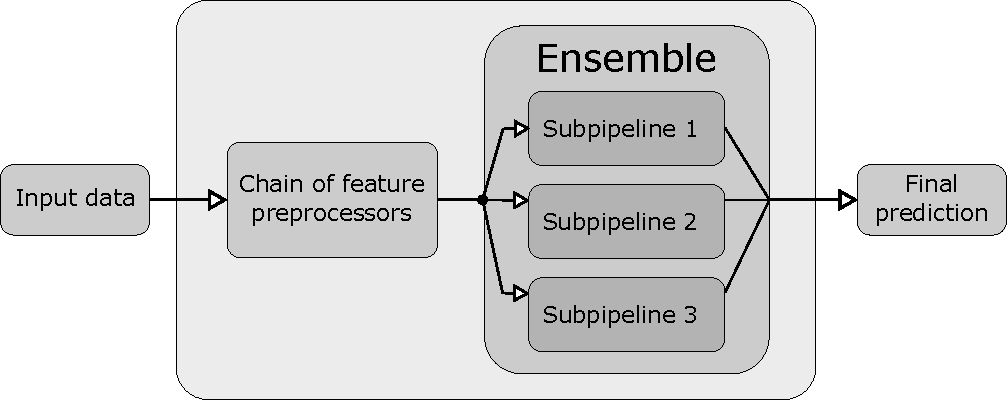
\includegraphics[width=0.7\textwidth]{../img/pipeline-pdfa.pdf}
\caption{Schema of an example pipeline}
\label{pic02:pipeline}
\end{figure}

The encoding is one of the most important parts of this system. The individual
represents a particular ML pipeline, which is composed of a chain of feature
preprocessing methods and of a final estimator. Additionally, we may allow
more complex pipeline steps like ensembles and complex feature
preprocessing methods like stacking or feature union (some of these methods are
described in the book by \cite{Brazdil:2008:MAD:1507541}). In such case, most of the
pipelines become in fact directed acyclic graphs (Figure~\ref{pic02:pipeline}).
Therefore, we cannot directly use the simple tree-based encoding. Instead we
use the developmental GP with cellular encoding described
in section~\ref{devGP}.

In our case, the embryo is an empty pipeline. To create a complex pipeline, we
modify it by inserting steps into it.

\begin{figure}[ht]\centering
    \subfloat[Tree encoding]{{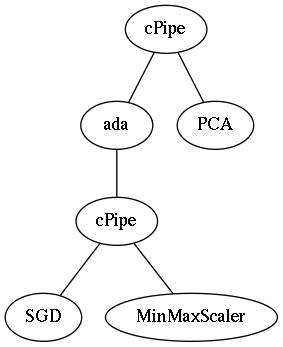
\includegraphics[width=0.25\textwidth]{../img/ada.png} }}%
    \qquad
    \subfloat[Encoded pipeline]{{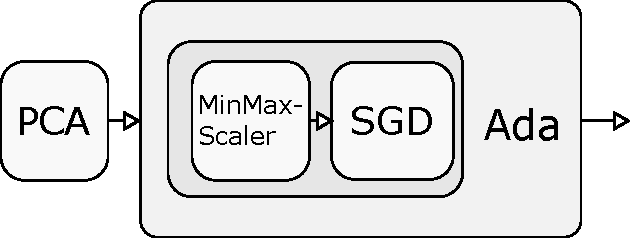
\includegraphics[width=0.5\textwidth]{../img/ada-pdfa.pdf} }}%
    \caption{An example pipeline encoded to a tree individual}%
    \label{pic:pipeencoding}%
\end{figure}

The process can be demonstrated on Figure
\ref{pic:pipeencoding}. The root of the tree represents the embryo which will
be modified by subsequent operations. In this case, the left subtree modifies
the ensemble structure whereas the right subtree modifies the feature
preprocessor chain. The pipeline contains only one preprocessor, hence the
right subtree is terminated by the corresponding node. The left child can be
either an ensemble or a simple method. Here it is the AdaBoost ensemble which
has one base classifier. The subestimator is again a pipeline, which is composed
of a MinMaxScaler and Stochastic gradient descent classifier. The specific
hyperparameter of every pipeline step are stored aside the nodes and are not
depicted in the figures.

\label{sec:decoding}
Table \ref{tab03:nodes} lists all nodes used in the current implementation of
our system. Input type is defined as a cartesian product of types, output type
is a single type; terminals have only the output type defined. Output types of
child nodes must match the input type of parent node. The list is extensible,
it is possible to add a definion of similar nodes, e.g. a different ensemble
flavour like stacking. The nodes that are specific for a given estimator
correspond to the list of methods in section \ref{tab03:methods}. To decode
the pipeline, the tree is traversed from root to leaves while applying the
operations associated with the nodes.

\begin{table}[b!]

\centering
\caption{Nodes representing modifying operations}\label{tab03:nodes}
\begin{tabular}{l c c p{0.38\textwidth}}
\toprule
\mc{\textbf{Node}\textsuperscript{1}} & \mc{\textbf{In type}\textsuperscript{2}} &
\mc{\textbf{Out type}\textsuperscript{3}} & \mc{\textbf{Operation}} \\
\midrule
cPipe       & $ens \times data$      & $out$  & Create pipeline with a preprocessor chain and a predictor \\
cPred       & $ens$                  & $out$  & Create pipeline only with a predictor \\
cData       & $featsel \times scale$ & $data$ & Create preprocessor chain with feature selector and scaler \\
cFeatSelect & $featsel$              & $data$ & Create preprocessor chain only with a feature selector \\
cScale      & $scale$                & $data$ & Create preprocessor chain only with a scaler \\
dUnion      & $data^n$               & $data$ & Create feature union in the preprocessor chain \\
\textit{ensemble} & $out^n$ & $ens$ & Insert ensemble \\
\textit{classifier} & $\emptyset$ & $out$ & Insert classifier \\
\textit{selector} & $\emptyset$ & $featsel$ & Insert feature selector \\
\textit{scaler} & $\emptyset$ & $scale$ & Insert scaler \\
\bottomrule

\multicolumn{4}{l}{\footnotesize
\textsuperscript{1}\textit{There is one specific node per ensemble, classifier
and preprocessor present}} \\

\multicolumn{4}{l}{\footnotesize
\textsuperscript{2}\textit{Variable arity is allowed (i.e. $n \in <1, max\_n>)$}} \\

\multicolumn{4}{l}{\footnotesize
\textsuperscript{3}\textit{In the last level classifier and preprocessing
can have output type $ens$ and $data$ resp.}} 

\end{tabular}

\end{table}

\subsection{Initialization} \label{sec:init}
As the initial population we grow $n$ trees where every tree has a random
height between 1 and overall maximum height. The tree is grown from root, which
is either a `cPipe' or `cPred' node (Table \ref{tab03:nodes}). Then, nodes are
inserted into the tree according to the input type of the parent. Before the
height limit is reached (during the \emph{growing phase}), both functions and
terminals are inserted into the tree. Then, only terminals are inserted to
keep the limit.

As terminals are inserted in the growing phase as well, the tree may become
smaller than the height limit. However, if the tree were built using the full
method, it would introduce a lot of feature preprocessing methods for taller
trees. Therefore, all node types listed in Table \ref{tab03:nodes} may be used
during the growing phase. Moreover, we define special terminal nodes which are
used only in the last level (\hyperref[tab03:nodes]{footnote 2}). It is
necessary to include them, as otherwise it would be impossible to finish the
tree in one level, but they would force the trees to be very short if used
during the growing phase.

\paragraph{Weighted selection}
During the node selection, we use weights to manage the probability of a node
to be chosen. The motivation is that some nodes represent lightweight methods
which have a short execution time, whereas some nodes slow down the evaluation
process, especially when present multiple times in the tree.

The process is as follows: every node is assigned to a group and each group has
a well defined weight. When selecting a node $n$ with output type $out$, we 
first determine all groups $G$ which correspond to any node with output type
$out$. Then we select a group $g$ from $G$ by a weighted random choice.
Finally, $n$ is selected by a simple random choice from $g$.

\paragraph{Variable arity}
Some nodes, e.g. ensemble nodes, may have a \emph{variable arity}. This means
that the actual arity is determined just when the node is about to be inserted
to the tree. The arity is determined by an interval which may or may not have
an upper bound. If the upper bound is not provided, it is usually limited by
a global arity limit to avoid bloat of the trees.

\paragraph{Method hyperparameters}
Every node has a list of possible values per hyperparameter associated with
it. During selection, the actual values are randomly selected from every list.
The validity is not verified in this phase, instead it is handled in the
evaluation phase \ref{genens:eval}.

\subsection{Genetic operators} \label{sec:repro}
In our system we use one type of crossover and three different types of
mutation. The crossover is the standard strongly typed subtree-swap operation.
The mutation operators will be described in more detail.

\paragraph{Subtree mutation}
As defined in section \ref{treeops}, in subtree mutation a chosen subtree is
replaced with a randomly generated tree. In our implementation we moreover
limit the height of the generated tree. For height $h$ of the subtree, the
height of the newly generated tree must be between $<1, h + \epsilon>$ for a
small value of $\epsilon$. This way we ensure that for small subtrees the new
subtree may be slightly higher and for big subtrees the overall height should
not increase too much.

\paragraph{Node swap mutation}
In this type of mutation, a randomly chosen node is replaced with a new node.
Both output and input types must match; if the new node supports variable
arity, all input types of the old node must satisfy the bounds. For this type
of mutation, any lower bound must be greater than zero.

\paragraph{Node argument mutation}
Mutates a hyperparameter of a random node --- chooses a new value from the list
of possible values. This method has many possible extensions which are more
described in section \ref{future} (future work).

\subsection{Fitness and selection} \label{sec:fitsel}
To compute the fitness, the individuals are decoded into scikit-learn 
pipelines as described in section \ref{sec:decoding} (individual encoding).
The specific machine learning methods which are used in the pipelines along
with evaluation details are listed in the following section.

The fitness has two objectives~---~evaluation score and logarithmized
evaluation time. The enviromental selection is done via NSGA-II and the 
parental selection is a tournament selection based on individual dominance and 
crowding distance. This approach allows us to prefer simpler yet
well-performing pipelines, as complex ensemble methods are typically
time-consuming. 

It may happen that some pipeline fails to run, for example due to an
unsupported hyperparameter combination. In that case, the individual is
discarded and a new one is generated. If the next individual is not valid
either, the process is repeated until a valid individual is generated.

\section{Evaluation and performance estimation} \label{genens:eval}
In this section we elaborate on the evaluation process. First we present the
pipelines and used methods in more detail. Then we present the evaluation and
a performance estimation method which was used to decrease the running time.

\subsection{Used machine learning methods} \label{tab03:methods}
We use the scikit-learn implementation of pipelines. An arbitrary pipeline
consists of multiple transformer steps and one predictor step, which is either
an ensemble or a base-learner. Any machine learning method that complies to the
scikit-learn API can act as a pipeline step \citep{sklearn_api}. Regression is
supported by the system as well, but in this work we focus only on
classification problems. Tables \ref{tab:clf}, \ref{tab:prepro} and
\ref{tab:ens} show all machine learning methods present in the default
configuration. Every method has a list of hyperparameter values associated
with it. These are optimized during the process of evolution;
if a hyperparameter is not present, it will be always set to its default value.

{\footnotesize
\begin{longtable}{l l}
\caption{Used classifiers with hyperparameters} \label{tab:clf} \\

\toprule
\multicolumn{2}{c}{\textbf{KNeighborsClassifier}} \\*
\midrule

n\_neighbors & [1, 2, 5] \\
algorithm & ['auto', 'ball\_tree', 'kd\_tree', 'brute'] \\

\midrule
\multicolumn{2}{c}{\textbf{LinearSVC}} \\*
\midrule

loss & [hinge,squared\_hinge] \\
penalty & [l1,l2] \\
C & [0.1,0.5,1.0,2,5,10,15] \\
tol & [0.0001,0.001,0.01] \\

\midrule
\multicolumn{2}{c}{\textbf{SVC}} \\*
\midrule

C & [0.1,0.5,1.0,2,5,10,15] \\
gamma & [scale,0.0001,0.001,0.01,0.1,0.5] \\
tol & [0.0001,0.001,0.01] \\

\midrule
\multicolumn{2}{c}{\textbf{LogisticRegression}} \\*
\midrule

penalty & [l1,l2] \\
C & [0.1,0.5,1.0,2,5,10,15] \\
tol & [0.0001,0.001,0.01] \\
solver & [newton-cg,lbfgs,liblinear,sag,saga] \\

\midrule
\multicolumn{2}{c}{\textbf{Perceptron}} \\*
\midrule

penalty & [None,l2,l1,elasticnet] \\
n\_iter & [1,2,5,10,100] \\
alpha & [0.0001,0.001,0.01] \\

\midrule
\multicolumn{2}{c}{\textbf{SGDClassifier}} \\*
\midrule

penalty & [none,l2,l1,elasticnet] \\
loss & [hinge,log,modified\_huber,squared\_hinge,perceptron] \\
max\_iter & [10,100,200] \\
tol & [0.0001,0.001,0.01] \\
alpha & [0.0001,0.001,0.01] \\
l1\_ratio & [0,0.15,0.5,1] \\
epsilon & [0.01,0.05,0.1,0.5] \\
learning\_rate & [constant,optimal] \\
eta0 & [0.01,0.1,0.5] \\
power\_t & [0.1,0.5,1,2] \\

\midrule
\multicolumn{2}{c}{\textbf{PassiveAggressiveClassifier}} \\*
\midrule

loss & [hinge,squared\_hinge] \\
C & [0.1,0.5,1.0,2,5,10,15] \\

\midrule
\multicolumn{2}{c}{\textbf{LinearDiscriminantAnalysis}} \\*
\midrule

solver & [lsqr,eigen] \\
shrinkage & [None,auto,0.1,0.5,1.0] \\\noalign{\penalty-5000}

\midrule
\multicolumn{2}{c}{\textbf{QuadraticDiscriminantAnalysis}} \\*
\midrule

reg\_param & [0.0,0.1,0.5,1] \\
tol & [0.0001,0.001,0.01] \\

\midrule
\multicolumn{2}{c}{\textbf{MLPClassifier}} \\*
\midrule

activation & [identity,logistic,relu] \\
solver & [lbfgs,sgd,adam] \\
alpha & [0.0001,0.001,0.01] \\
learning\_rate & [constant,invscaling,adaptive] \\
tol & [0.0001,0.001,0.01] \\
max\_iter & [10,100,200] \\
learning\_rate\_init & [0.0001,0.001,0.01] \\
power\_t & [0.1,0.5,1,2] \\
momentum & [0.1,0.5,0.9] \\
hidden\_layer\_sizes & [(100,),(50,),(20,),(10,)] \\

\midrule
\multicolumn{2}{c}{\textbf{DecisionTreeClassifier}} \\*
\midrule

criterion & [gini,entropy] \\
max\_features & [0.05,0.1,0.25,0.5,0.75,1] \\
max\_depth & [1,2,5,10,15,25,50,100] \\
min\_samples\_split & [2,5,10,20] \\
min\_samples\_leaf & [1,2,5,10,20] \\

\midrule
\multicolumn{2}{c}{\textbf{GaussianNB}} \\*
\midrule
\multicolumn{2}{c}{\textit{-}} \\

\midrule
\multicolumn{2}{c}{\textbf{GradientBoostingClassifier}} \\*
\midrule

loss & [deviance,exponential] \\
n\_estimators & [20,50,100,200] \\
subsample & [0.3,0.5,0.75,1.0] \\


\midrule
\multicolumn{2}{c}{\textbf{RandomForestClassifier}} \\*
\midrule

n\_estimators & [10,50,100,150,200] \\


\midrule
\multicolumn{2}{c}{\textbf{ExtraTreesClassifier}} \\*
\midrule

n\_estimators & [10,50,100,150,200] \\


\bottomrule

\end{longtable}
}

{\footnotesize
\begin{longtable}{l l}

\caption{Used preprocessors with hyperparameters} \label{tab:prepro} \\

\midrule
\multicolumn{2}{c}{\textbf{NMF}} \\*
\midrule

feat\_frac & [0.01,0.05,0.1,0.25,0.5,0.75,1] \\
solver & [cd,mu] \\

\midrule
\multicolumn{2}{c}{\textbf{FactorAnalysis}} \\*
\midrule

feat\_frac & [0.01,0.05,0.1,0.25,0.5,0.75,1] \\

\midrule
\multicolumn{2}{c}{\textbf{FastICA}} \\*
\midrule

feat\_frac & [0.01,0.05,0.1,0.25,0.5,0.75,1] \\

\midrule
\multicolumn{2}{c}{\textbf{PCA}} \\*
\midrule

feat\_frac & [0.01,0.05,0.1,0.25,0.5,0.75,1] \\
whiten & [False,True] \\

\midrule
\multicolumn{2}{c}{\textbf{SelectKBest}} \\*
\midrule

feat\_frac & [0.01,0.05,0.1,0.25,0.5,0.75,1] \\
score\_func & [feature\_selection.chi2,feature\_selection.f\_classif] \\

\midrule
\multicolumn{2}{c}{\textbf{MaxAbsScaler}} \\*
\midrule
\multicolumn{2}{c}{\textit{-}} \\

\midrule
\multicolumn{2}{c}{\textbf{MinMaxScaler}} \\*
\midrule
\multicolumn{2}{c}{\textit{-}} \\

\midrule
\multicolumn{2}{c}{\textbf{Normalizer}} \\*
\midrule
\multicolumn{2}{c}{\textit{-}} \\

\midrule
\multicolumn{2}{c}{\textbf{StandardScaler}} \\*
\midrule
\multicolumn{2}{c}{\textit{-}} \\

\bottomrule \\[-8pt]
\multicolumn{2}{p{0.8\linewidth}}{Note: \emph{feat\_frac} is an artificial
feature which represents a fraction of total feature count; it is converted
to \emph{n\_components} or \emph{k} respectively}

\end{longtable}
}


%\begin{table}


{ \footnotesize
\begin{longtable}{>{\itshape}l l}

\caption{Used ensembles with hyperparameters} \label{tab:ens} \\

\toprule
\multicolumn{2}{c}{\textbf{AdaBoostClassifier}} \\*
\midrule

n\_estimators & [5, 10, 50, 100, 200] \\
algorithm & [SAMME, SAMME.R] \\

\midrule
\multicolumn{2}{c}{\textbf{BaggingClassifier}} \\*
\midrule

n\_estimators & [5, 10, 50, 100, 200] \\

\midrule
\multicolumn{2}{c}{\textbf{VotingClassifier}} \\*
\midrule

voting & [hard]\\

\bottomrule

\end{longtable}
}
%\end{table}

 
\subsection{Scoring and sampling} \label{sec:scoresample}
The score is computed by running the pipeline on the dataset using the
scikit-learn scorer interface. The default score is predictive accuracy,
but other metrics are supported as well. There are multiple evaluation
strategies to choose from --- the default strategy is k-fold cross-validation,
but it is also possible to specify a separate validation set for scoring.
% TODO cite scorer

If the number of examples is small enough, it is possible to use the whole
dataset for evaluation. On larger datasets though, the duration time may be
too long even for a small number of fitness evaluations.
As such, it is necessary to decrease the evaluation time of a single pipeline.
We use one of the performance estimation methods mentioned in section
\ref{sec:modelarch} --- evaluation on smaller subsets of data.

The strategy is as follows: we generate stratified random samples of the
original dataset. The samples are either generated per generation or per
every fitness evaluation, while the latter has proved to be more effective. A
possible explanation is that if we generate only one sample per generation,
we cannot ensure that it is representative enough. Thus, the individuals which
score particularly well on this sample may not generalize well. The second
approach suffers from this problem as well, but since we generate a sample
per evaluation, every individual has a fair chance of getting a good sample.
Possible improvements of this approach are presented in section \ref{future}.

As the samples are typically much smaller than the whole dataset, the score
is computed as a (stratified) k-fold cross-validation on a sample.
\section{Implementation} \label{genens:impl}
The source code of our system is available in a public GitHub repository
\citep{git_genens}.
For the machine-learning side of the implementation we used scikit-learn
\citep{scikit-learn}.

We extended the Pipeline class in order to enable usage
of pipelines as base-learners (some ensembles require \texttt{predict\_proba}
which is not available on standard pipelines). A meta-transformer was also
added to provide conversion between \texttt{feat\_frac} and 
\texttt{n\_components} or \texttt{k} hyperparameters respectively (as reflected
in Table \ref{tab:prepro}).

The components of the evolutionary algorithm were managed by the tools provided by
the library DEAP \citep{DEAP_JMLR2012}. However, although DEAP supports genetic
programming, the primitives cannot be created with variable arity, hence we
reimplemented the concept.
For parallelization of fitness evaluations we used the library Joblib
\citep{joblib}.

% TODO timeouts cite lib (+ check if any other libraries like that)

\subsection{Configurability}
The system can be customised by following configuration hyperparameters:

\begin{itemize}
\item population size
\item number of generations
\item maximum tree height
\item maximum arity (global for all nodes)
\item timeout per individual evaluation (results in invalid score)
\item evaluation strategy
\item recombination probabilities from algorithm \ref{alg:devgp}
\item custom scorer (according to scikit-learn API)
\end{itemize}



% o chap 4
% exper.

% exp - evaluace - per gen, per ind, cele  10x 10 fold cv (train test?)
%    --- schovat kappu

% V patek rozmyslet experiment
% probs & wilt + small, big dataset

% popsat ten velky, jako posledni experiment
% porovnani ja vs max z openml
% popsat...
% boxplot,...
% cil je jestli to funguje...
% presne nastaveni. Vsechno. Na githubu mit to nstaveni, zkopirovat configy

% zeptat na obrazky, az to vygeneruju

% patek Conclus, Intro


% Cil, nastaveni, vysledky tabulka obrazek jedinec; koment, co je videt, ukazali jsme co jsme chteli?

\chapter*{Conclusion}
\addcontentsline{toc}{chapter}{Conclusion}

The main result of our work is the design of an AutoML system for automatic
supervised learning pipeline optimization. Using the developmental GP, we created a general encoding
of scikit-learn pipelines that converts a DAG pipeline into a tree representation.

The encoding was designed in an extensible way. The list of used methods can be easily 
extended with more ensembles and methods that comply to the scikit-learn API.
We also implemented a tree individual that, compared to the DEAP tree individual, supports
variable arity of nodes.

We introduced several bloat-reducing approaches. The grow method of the GP was
modified to initialize less branched trees, which were more suitable for representation
of pipelines. We also employed a weighted node selection, which prefers simpler methods.
That way, we avoided nested ensembles which are computationally demanding, but do not
significantly improve the score. 

To decrease the running time of the optimization, we implemented some performance
estimation strategies based on sampling. A sample of the input dataset was either
created once per generation or per individual evaluation. The two strategies were
then tested in the first experiment on two medium size dataset and one large dataset.
The results of the experiment did not show any noticeable difference in
the two approaches, but implied that by generating a sample for every evaluation, we
increase the variance of results.

For the evolutionary optimization itself, we designed specific genetic operators. The
subtree crossover and subtree mutation greatly alter the structure of the pipeline.
The point mutation changes only one method of the pipeline while preserving the
architecture. Finally, the node argument mutation changes a random hyperparameter of
a random node, thus targeting the CASH problem.

To test whether the absence of a certain genetic operator influences the final result,
we carried out the second experiment, where we turned the operators off one at a time.
With this settings, we have done several runs on a small dataset and on a medium sized
unbalanced dataset. The results of the experiments have shown that on the medium
sized dataset, the hyperparameter mutation is essential for obtaining good results.
On the second dataset, turning off the point mutation produced significantly better
results. This behaviour is to be subject of future research. Finally, in all cases
the results were better than the simple case where all genetic operators were turned
off.

In the last experiment, we evaluated the performance on the system on the OpenML-CC18 benchmark suite.
We ran the evolutionary optimization on each of the 72 datasets of the
benchmark, while using one of the sampling strategies. Three best pipelines were evaluated
and the maximum of the scores was chosen as the final output. We then compared our
results with the statistic of runs uploaded to OpenML. Overall, on most datasets
our system performed better than the upper quartile of OpenML runs or only slightly
below it. In one case, our system outperformed all runs uploaded to OpenML.

In future extensions of our system, there are several concepts which are to be
explored. As has been shown in the second experiment, the mutation of hyperparameters
may significantly improve the results. As such, it would be suitable to employ a
better optimization strategy that a simple selection of values from a list. One
possibility would be to use the evolutionary strategies, which is a subfield of
evolutionary algorithms particularly suited for continuous optimization. Another
option is to create a Bayesian optimization method inspired by existing AutoML
systems. Moreover, some additional methods may yield promising results, notably
hill-climbing or mutation of multiple hyperparameters at once.
As shown in experiment 2, it is necessary to further optimize the genetic operators.
Again, more sophisticated methods could lead to interesting pipeline architectures.
A related problem is the setting of weights used for initialization, which should be
thoroughly explored.

To extend the methods used in the pipelines, a stacking estimator should be added
to the primitive set, as it may lead to very promising results. Also, we should focus
more on the data preprocessing methods, as users of this system still need to perform
some initial encoding and imputation of missing data. Our system should be then
compared with existing AutoML methods on suitable benchmark data.



% Future work

% focus more on the data preprocessing part
% fut work - time measurements

%%% Bibliography
%%% Bibliography (literature used as a source)
%%%
%%% We employ bibTeX to construct the bibliography. It processes
%%% citations in the text (e.g., the \cite{...} macro) and looks up
%%% relevant entries in the bibliography.bib file.
%%%
%%% The \bibliographystyle command selects, which style will be used
%%% for references from the text. The argument in curly brackets is
%%% the name of the corresponding style file (*.bst). Both styles
%%% mentioned in this template are included in LaTeX distributions.

\bibliographystyle{plainnat}    %% Author (year)
% \bibliographystyle{unsrt}     %% [number]

\renewcommand{\bibname}{Bibliography}

%%% Generate the bibliography. Beware that if you cited no works,
%%% the empty list will be omitted completely.

\bibliography{bibliography}

%%% If case you prefer to write the bibliography manually (without bibTeX),
%%% you can use the following. Please follow the ISO 690 standard and
%%% citation conventions of your field of research.

% \begin{thebibliography}{99}
%
% \bibitem{lamport94}
%   {\sc Lamport,} Leslie.
%   \emph{\LaTeX: A Document Preparation System}.
%   2nd edition.
%   Massachusetts: Addison Wesley, 1994.
%   ISBN 0-201-52983-1.
%
% \end{thebibliography}


%%% Algorithms used in the thesis.
\listofalgorithms

%%% Figures used in the thesis (consider if this is needed)
\listoffigures

%%% Tables used in the thesis (consider if this is needed)
%%% In mathematical theses, it could be better to move the list of tables to the beginning of the thesis.
\listoftables

%%% Abbreviations used in the thesis, if any, including their explanation
%%% In mathematical theses, it could be better to move the list of abbreviations to the beginning of the thesis.
\chapwithtoc{List of Abbreviations}

%%% Attachments to the bachelor thesis, if any. Each attachment must be
%%% referred to at least once from the text of the thesis. Attachments
%%% are numbered.
%%%
%%% The printed version should preferably contain attachments, which can be
%%% read (additional tables and charts, supplementary text, examples of
%%% program output, etc.). The electronic version is more suited for attachments
%%% which will likely be used in an electronic form rather than read (program
%%% source code, data files, interactive charts, etc.). Electronic attachments
%%% should be uploaded to SIS and optionally also included in the thesis on a~CD/DVD.
%%% Allowed file formats are specified in provision of the rector no. 72/2017.
\appendix
\chapter{Attachments}

\section{First Attachment}

\openright
\end{document}
